\documentclass[letterpaper, 10pt, conference]{ieeeconf}
%\documentclass[10pt,english,a4paper]{IEEEtran}
\IEEEoverridecommandlockouts
\overrideIEEEmargins

%\usepackage[a4paper, total={14cm, 25cm}]{geometry}
\usepackage{blindtext}
\usepackage[utf8]{inputenc}
\usepackage{amsmath}
\usepackage{amssymb}
\usepackage{color}
\usepackage{graphicx}
\usepackage[pdfencoding=auto]{hyperref}
%\usepackage{natbib}
\usepackage{bm}
\usepackage{graphicx}
\usepackage{comment}
\usepackage{soul}
\usepackage{pdfpages}
%\usepackage[pdftex]{graphicx}
\usepackage{subfigure}
\pdfminorversion=4


\sethlcolor{green}

% custom commands
% \newcommand{\colvec}[1]{\left[\begin{array}{c} #1 \end{array}\right]}
% => use {bmatrix} from amsmath
%    \begin{bmatrix} a \\ b \\ c \end{bmatrix}
\newcommand{\dd}[1]{\ensuremath {{\rm d}{#1}}}
\newcommand{\defeq}{\stackrel{\mathrm{def}}{=}}
% \newcommand{\defeq}{\stackrel{\text{def}}{=}}
% \newcommand{\defeq}{:=}
\newcommand{\diag}{\mathrm{diag}}
\newcommand{\tr}{\mathrm{tr}}
\renewcommand{\th}[1]{\ensuremath {#1}^{\textrm{th}}}
\renewcommand{\vec}[1]{\ensuremath \overrightarrow{#1}}

% velocities
\def\alphad{\dot{\alpha}}
\def\betad{\dot{\beta}}
\def\bfcd{\dot{\bfc}}
\def\bfpd{\dot{\bfp}}
\def\bfqd{\dot{\bfq}}
\def\bfrd{\dot{\bfr}}
\def\bfxid{\dot{\bfxi}}
\def\omegad{\dot{\omega}}
\def\rd{\dot{r}}
\def\sd{\dot{s}}
\def\xd{\dot{x}}
\def\yd{\dot{y}}
\def\zd{\dot{z}}

% accelerations
\def\alphadd{\ddot{\alpha}}
\def\betadd{\ddot{\beta}}
\def\bfcdd{\ddot{\bfc}}
\def\bfpdd{\ddot{\bfp}}
\def\bfqdd{\ddot{\bfq}}
\def\bfrdd{\ddot{\bfr}}
\def\rdd{\ddot{r}}
\def\sdd{\ddot{s}}
\def\xdd{\ddot{x}}
\def\ydd{\ddot{y}}
\def\zdd{\ddot{z}}

% bold greek lowercase letters
\newcommand{\bfalpha}{\boldsymbol{\alpha}}
\newcommand{\bfbeta}{\boldsymbol{\beta}}
\newcommand{\bfgamma}{\boldsymbol{\gamma}}
\newcommand{\bfdelta}{\boldsymbol{\delta}}
\newcommand{\bfepsilon}{\boldsymbol{\epsilon}}
\newcommand{\bfzeta}{\boldsymbol{\zeta}}
\newcommand{\bfeta}{\boldsymbol{\eta}}
\newcommand{\bftheta}{\boldsymbol{\theta}}
\newcommand{\bfiota}{\boldsymbol{\iota}}
\newcommand{\bfkappa}{\boldsymbol{\kappa}}
\newcommand{\bflambda}{\boldsymbol{\lambda}}
\newcommand{\bfmu}{\boldsymbol{\mu}}
\newcommand{\bfnu}{\boldsymbol{\nu}}
\newcommand{\bfxi}{\boldsymbol{\xi}}
\newcommand{\bfomicron}{\boldsymbol{\omicron}}
\newcommand{\bfpi}{\boldsymbol{\pi}}
\newcommand{\bfrho}{\boldsymbol{\rho}}
\newcommand{\bftau}{\boldsymbol{\tau}}
\newcommand{\bfupsilon}{\boldsymbol{\upsilon}}
\newcommand{\bfphi}{\boldsymbol{\phi}}
\newcommand{\bfchi}{\boldsymbol{\chi}}
\newcommand{\bfpsi}{\boldsymbol{\psi}}
\newcommand{\bfomega}{\boldsymbol{\omega}}

% bold greek letters
\newcommand{\bfAlpha}{\boldsymbol{\Alpha}}
\newcommand{\bfBeta}{\boldsymbol{\Beta}}
\newcommand{\bfGamma}{\boldsymbol{\Gamma}}
\newcommand{\bfDelta}{\boldsymbol{\Delta}}
\newcommand{\bfEpsilon}{\boldsymbol{\Epsilon}}
\newcommand{\bfZeta}{\boldsymbol{\Zeta}}
\newcommand{\bfEta}{\boldsymbol{\Eta}}
\newcommand{\bfTheta}{\boldsymbol{\Theta}}
\newcommand{\bfIota}{\boldsymbol{\Iota}}
\newcommand{\bfKappa}{\boldsymbol{\Kappa}}
\newcommand{\bfLambda}{\boldsymbol{\Lambda}}
\newcommand{\bfMu}{\boldsymbol{\Mu}}
\newcommand{\bfNu}{\boldsymbol{\Nu}}
\newcommand{\bfXi}{\boldsymbol{\Xi}}
\newcommand{\bfOmicron}{\boldsymbol{\Omicron}}
\newcommand{\bfPi}{\boldsymbol{\Pi}}
\newcommand{\bfRho}{\boldsymbol{\Rho}}
\newcommand{\bfTau}{\boldsymbol{\Tau}}
\newcommand{\bfUpsilon}{\boldsymbol{\Upsilon}}
\newcommand{\bfPhi}{\boldsymbol{\Phi}}
\newcommand{\bfChi}{\boldsymbol{\Chi}}
\newcommand{\bfPsi}{\boldsymbol{\Psi}}
\newcommand{\bfOmega}{\boldsymbol{\Omega}}

% bold lowercase letters
\newcommand{\bfa}{\ensuremath {\bm{a}}}
\newcommand{\bfb}{\ensuremath {\bm{b}}}
\newcommand{\bfc}{\ensuremath {\bm{c}}}
\newcommand{\bfd}{\ensuremath {\bm{d}}}
\newcommand{\bfe}{\ensuremath {\bm{e}}}
\newcommand{\bff}{\ensuremath {\bm{f}}}
\newcommand{\bfg}{\ensuremath {\bm{g}}}
\newcommand{\bfh}{\ensuremath {\bm{h}}}
\newcommand{\bfi}{\ensuremath {\bm{i}}}
\newcommand{\bfj}{\ensuremath {\bm{j}}}
\newcommand{\bfk}{\ensuremath {\bm{k}}}
\newcommand{\bfl}{\ensuremath {\bm{l}}}
\newcommand{\bfm}{\ensuremath {\bm{m}}}
\newcommand{\bfn}{\ensuremath {\bm{n}}}
\newcommand{\bfo}{\ensuremath {\bm{o}}}
\newcommand{\bfp}{\ensuremath {\bm{p}}}
\newcommand{\bfq}{\ensuremath {\bm{q}}}
\newcommand{\bfr}{\ensuremath {\bm{r}}}
\newcommand{\bfs}{\ensuremath {\bm{s}}}
\newcommand{\bft}{\ensuremath {\bm{t}}}
\newcommand{\bfu}{\ensuremath {\bm{u}}}
\newcommand{\bfv}{\ensuremath {\bm{v}}}
\newcommand{\bfw}{\ensuremath {\bm{w}}}
\newcommand{\bfx}{\ensuremath {\bm{x}}}
\newcommand{\bfy}{\ensuremath {\bm{y}}}
\newcommand{\bfz}{\ensuremath {\bm{z}}}

% bold uppercase letters
\newcommand{\bfA}{\mathbf{A}}
\newcommand{\bfB}{\mathbf{B}}
\newcommand{\bfC}{\mathbf{C}}
\newcommand{\bfD}{\mathbf{D}}
\newcommand{\bfE}{\mathbf{E}}
\newcommand{\bfF}{\mathbf{F}}
\newcommand{\bfG}{\mathbf{G}}
\newcommand{\bfH}{\mathbf{H}}
\newcommand{\bfI}{\mathbf{I}}
\newcommand{\bfJ}{\mathbf{J}}
\newcommand{\bfK}{\mathbf{K}}
\newcommand{\bfL}{\mathbf{L}}
\newcommand{\bfM}{\mathbf{M}}
\newcommand{\bfN}{\mathbf{N}}
\newcommand{\bfO}{\mathbf{O}}
\newcommand{\bfP}{\mathbf{P}}
\newcommand{\bfQ}{\mathbf{Q}}
\newcommand{\bfR}{\mathbf{R}}
\newcommand{\bfS}{\mathbf{S}}
\newcommand{\bfT}{\mathbf{T}}
\newcommand{\bfU}{\mathbf{U}}
\newcommand{\bfV}{\mathbf{V}}
\newcommand{\bfW}{\mathbf{W}}
\newcommand{\bfX}{\mathbf{X}}
\newcommand{\bfY}{\mathbf{Y}}
\newcommand{\bfZ}{\mathbf{Z}}

% caligraphic uppercase letters
\newcommand{\calA}{{\cal A}}
\newcommand{\calB}{{\cal B}}
\newcommand{\calC}{{\cal C}}
\newcommand{\calD}{{\cal D}}
\newcommand{\calE}{{\cal E}}
\newcommand{\calF}{{\cal F}}
\newcommand{\calG}{{\cal G}}
\newcommand{\calH}{{\cal H}}
\newcommand{\calI}{{\cal I}}
\newcommand{\calJ}{{\cal J}}
\newcommand{\calK}{{\cal K}}
\newcommand{\calL}{{\cal L}}
\newcommand{\calM}{{\cal M}}
\newcommand{\calN}{{\cal N}}
\newcommand{\calO}{{\cal O}}
\newcommand{\calP}{{\cal P}}
\newcommand{\calQ}{{\cal Q}}
\newcommand{\calR}{{\cal R}}
\newcommand{\calS}{{\cal S}}
\newcommand{\calT}{{\cal T}}
\newcommand{\calU}{{\cal U}}
\newcommand{\calV}{{\cal V}}
\newcommand{\calW}{{\cal W}}
\newcommand{\calX}{{\cal X}}
\newcommand{\calY}{{\cal Y}}
\newcommand{\calZ}{{\cal Z}}

% blackboard uppercase letters
\newcommand{\bbA}{{\mathbb{A}}}
\newcommand{\bbB}{{\mathbb{B}}}
\newcommand{\bbC}{{\mathbb{C}}}
\newcommand{\bbD}{{\mathbb{D}}}
\newcommand{\bbE}{{\mathbb{E}}}
\newcommand{\bbF}{{\mathbb{F}}}
\newcommand{\bbG}{{\mathbb{G}}}
\newcommand{\bbH}{{\mathbb{H}}}
\newcommand{\bbI}{{\mathbb{I}}}
\newcommand{\bbJ}{{\mathbb{J}}}
\newcommand{\bbK}{{\mathbb{K}}}
\newcommand{\bbL}{{\mathbb{L}}}
\newcommand{\bbM}{{\mathbb{M}}}
\newcommand{\bbN}{{\mathbb{N}}}
\newcommand{\bbO}{{\mathbb{O}}}
\newcommand{\bbP}{{\mathbb{P}}}
\newcommand{\bbQ}{{\mathbb{Q}}}
\newcommand{\bbR}{{\mathbb{R}}}
\newcommand{\bbS}{{\mathbb{S}}}
\newcommand{\bbT}{{\mathbb{T}}}
\newcommand{\bbU}{{\mathbb{U}}}
\newcommand{\bbV}{{\mathbb{V}}}
\newcommand{\bbW}{{\mathbb{W}}}
\newcommand{\bbX}{{\mathbb{X}}}
\newcommand{\bbY}{{\mathbb{Y}}}
\newcommand{\bbZ}{{\mathbb{Z}}}


\def\ankle{\text{ankle}}
\newcommand{\TODO}[1]{{\color{red} {\bf TODO:} {#1}}}
\newcommand{\SC}[1]{{\color{red} {\bf SC:} {#1}}}
\renewcommand{\SS}[1]{{\color{blue} {\bf SC:} {#1}}}
\newcommand\norm[1]{\left\lVert#1\right\rVert}
%\renewcommand\IEEEkeywordsname{Keywords}

\def\pcmd{p^{cmd}}
\def\vcmd{v^{cmd}}

\title{\Large \bf
	Wheel Kinematics and Dynamics}

\author{Saeid Samadi, and Abderrahmane Kheddar
	\thanks{Authors are with Montpellier Laboratory of Informatics,
		Robotics and Microelectronics (LIRMM), CNRS-University of Montpellier, France.
		Corresponding author: {\tt\footnotesize saeid.samadi@lirmm.fr}}
}

\begin{document}

\maketitle
\thispagestyle{empty}
\pagestyle{empty}

\begin{abstract}
	This study deals with the kinematic and dynamic model of wheels. Wheels are part of robot model and this modeling has a significant effect in the performance of the robot...
\end{abstract}

\begin{keywords}
	Wheeled Robot Model, Dynamics, Kinematics
\end{keywords}

	
%%% XXX To be uncommented on "ieeeConf" document class
%\begin{keywords}
%Chebyshev center
%\end{keywords}
\begin{comment}

\begin{table}[h]
\renewcommand{\arraystretch}{1.5}
\caption{Table of Symbols}
\label{table_example}
\centering
\begin{tabular}{p{0.09\textwidth}|p{0.09\textwidth}||p{0.09\textwidth}|p{0.09\textwidth}}
%\begin{tabular*}{0.4\textwidth}{l | r || l | r}
\hline
\bfseries \centering First & \bfseries Next & me & you \\
\hline\hline
1.0 & 2.0\\
\hline
\end{tabular}
\end{table}
\end{comment}

\section{Introduction} \label{Sec_Introduction}

We characterize the robot or vehicle wheels into:
\begin{itemize}
	\item Driving wheel
	\item Push-pull wheel
\end{itemize}

The driving wheel has a torque input $\tau_{in}$ at the center of mass which is translated from the driving shaft. On the other hand, a linear force is applying to the CoM of a push/pull wheel. The Normal force $N$ is same in the both wheels acting on the driving/push-pull contact points with the ground $Q_{d/p}$. On the other hand, the friction forces $f_{fr}$ on these two types has different directions and cause contrary effects.

\TODO{add wheel figures}

Note that the friction force on the driving wheel, is pointing to the $(+x)$ and for the push/pull wheel, the direction is $(-x)$. For the driving wheel, $f_{fr}$ causes forward movement and $tau_{in}$ results in rolling. Whereas for the push/pull wheel, moving forward and rolling are results of $P_{in}$ and $f_{fr}$ respectively.

The effect of the torques and forces on the motion of a wheel can also be categorized into:
\begin{itemize}
\item Driving Component
\item Rolling Component
\item Normal Component
\end{itemize}

The forces/torques which result in the forward/backward driving of the wheel are among \emph{driving components}. For a driving wheel, friction force and for a push/pull wheel, the input force are driving components. On the other hand, forces/torques which result in rolling motion of the wheel are categorized as rolling components; such as input torque and friction force for driving and push-pull wheels, respectively.

The normal component is also including the forces which are normal to the direction of the linear motion and has no effect on driving and rolling motions of the wheel.
\section{Driving Wheel On the Flat Surface} \label{DrivingWheel}

Assume that the wheel is driven by driving torque $\tau_{in}$ without any active pulling forces $P_{in}$ (\textcolor{red}{Fig}). This type of wheel is noted as pure driving wheel in the rest of the paper. We need to identify a valid condition for slippage. 

\subsection{Slippage Criteria for a Driving Wheel} \label{SlipCri-DW}

For a pure driving wheel, the decisive variable is the amount of $\tau_{in}$. If $\tau_{in}$ is less than a maximum value of $\tau_{in}^{max}$, then the motion is without slippage. Otherwise, wheel's motion is a combination of rolling and slipping. For a driving wheel, we have the following relations:
\begin{align}
F_{fr} &= ma_c \label{f_fr}\\
\tau_{in} - F_{fr} &= I_c \alpha \label{moment_eq}
\end{align}

Assuming no slippage condition and considering the maximum possible static force before slippage, we have:
\begin{align}
F_{fr}^{max} &= \mu_{s} N \label{f_fr_max} \\
\alpha &= \frac{a_c}{R} \label{alpha_noSlip}
\end{align}
where $\mu_s$ and $R$ are the static friction coefficient and wheel radius. Subsequently, we note he dynamic friction coefficient as $\mu_d$. from~\eqref{f_fr}~and~\eqref{f_fr_max}, we have:
\begin{align}
a_c^{max} = \frac{F_{fr}^{max}}{m} = \mu_s g
\end{align}
Therefore the maximum input torque to the wheel before starting the slippage is calculated from~\eqref{moment_eq}:
\begin{align}
\tau_{in}^{max} = I_c \frac{a_c^{max}}{R} + R F_{fr}^{max}
\end{align}
So, the slippage condition for a driving wheel on the flat surface is:
\begin{align}
if \begin{cases}
\tau_{in} \leqslant \tau_{in}^{max} &\Rightarrow \ \text{No Slip} \\
\text{Otherwise} &\Rightarrow \ \text{Slip}
\end{cases} \label{slipCondition}
\end{align}
In the following two subsections, we are analyzing the wheel dynamics in absence and presence of the slippage.
\subsection{Driving Wheel Without Slippage}
As described in~\eqref{slipCondition}, the condition for no slippage is $\tau_{in} \leqslant \tau_{in}^{max}$. Using~\eqref{f_fr},\eqref{moment_eq}~and~\eqref{alpha_noSlip} we have:
\begin{align*}
\tau_{in} - ma_c &= I_c \frac{a_c}{R} \\
\Rightarrow \tau_{in} &= (\frac{I_c}{R} + m)a_c
\end{align*}
so then:
\begin{align}
a_c = \frac{\tau_{in}}{\frac{I_c}{R} + m}
\end{align}
So $\alpha = \frac{a_c}{R}$ is calculated accordingly and the other components at time $t$ are:
\begin{align}
v_{c,t} &= a_{c,t}dt + v_{c,t-dt} \label{linearVel}\\
\omega_{c,t} &= \alpha_{c,t}dt + \omega_{c,t-dt} \label{angularVel}\\
F_{fr} &= ma_c
\end{align}
where $dt$ denotes the duration of each time step. Note that the value of the $F_{fr}$ is not equal to $\mu_sN$ except when it reaches to the slipping limit.

In order to calculate the velocity of each point on the wheel as a rigid body with respect to the inertial frame shown in \textcolor{red}{Fig1}, we use the relative velocity equation. The relative velocity of a point such as $K$ with respect to the inertial frame is $v_{K/O}$ and for simplicity, it is noted as $v_K$.
\begin{align}
v_Q = v_{Q/c} + v_c
\end{align}
At a specific time, the point $Q$ is a selected as the contact point of the wheel with the ground and fixed to the wheel. By considering no slippage condition, $v_c = R\omega$ and $v_{Q/c} = -R\omega$. So then the velocity of point $Q$ with respect to the inertial frame is becoming $0$.

\TODO{fig2}

If case of $R\omega \neq v_c$, slip occurs. This slippage can be a \emph{forward or backward slippage}. For better imagination of the expression Forward slippage, we can consider a wheel without rolling (or full-brake) and pushing forward. What happens is a pure slippage without any rotation and called Forward slippage. On the other hand, if the wheel just has the rotation in place (without linear velocity), then Backward slippage occurs.

\textcolor{red}{Fig3}
\subsection{Driving Wheel With Slippage}
For a driving wheel, $R\omega > v_c$ is possible. This can happen if $\tau_{in} > \tau_{in}^{max}$. In that case, the contact point is slightly sliding on the ground along with the rotary motion of the wheel. So the friction force becomes $F_{fr} = \mu_d N$:
\begin{align}
F_{fr} &= \mu_d mg = ma_c \\
\Rightarrow a_c &= \mu_dg \\
\tau_{in} - ma_c &= I_c \alpha \\
\Rightarrow \alpha &= \frac{\tau_{in} - ma_c}{I_c}
\end{align}
Then the linear and angular velocities can be computed same as~\eqref{linearVel}~and~\eqref{angularVel}.

\section{Push-pull Wheel On the Flat Surface}
A push-pull wheel is driven by an exogenous pulling or pushing force $P_{in}$. Therefore, this force is the driving component and the friction force which has the opposite direction, will be the rolling component. In this section, we study the pure push/pull wheel without applying any exogenous torque inputs.

\subsection{Slippage Criteria for a Push-Pull Wheel} \label{SlipCri-PW}
\subsection{Push-Pull Wheel Without Slippage}
\subsection{Push-Pull Wheel With Slippage}


\section{Parametric Computation of the Point Velocities on the Wheel}
\textcolor{red}{Figs: Fig4, Figures of the position of the points on the wheel wrt time}
\section{Generic Scenarios}
\subsection{Wheel on the tilted surface}

\begin{comment}
Wheel kinematics and dynamics are widely studied. Considering the multi-directional slippages, due to numerous variables such as wheel inertia, material and contact forces within these models, are challenging.  In sections~\ref{Sec_Kinematics}~and~\ref{Sec_Dynamics}, we describe the proposed method in~\cite{Seegmiller2014thesis}.
\section{Wheel Kinematics} \label{Sec_Kinematics}

The case study for~\cite{Seegmiller2014thesis} is a car model with six wheels as shown in Fig.~\eqref{rocky7}
\begin{figure}[!h] 
	\centering
	\subfigure[]{
		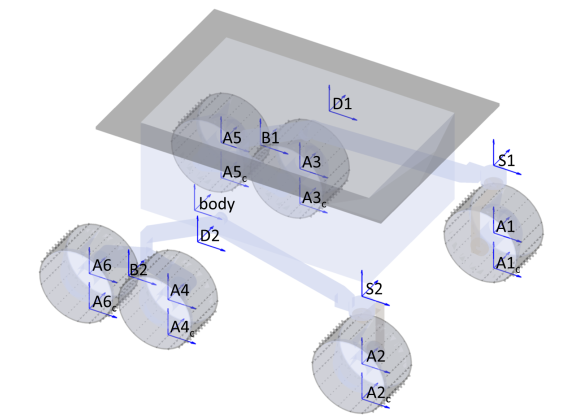
\includegraphics[width= 0.65\columnwidth]{figs/car.png}
		\label{Choreonoid}
	} 
	\subfigure[]{
		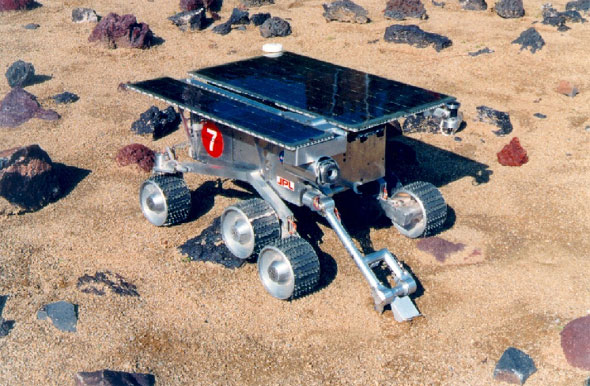
\includegraphics[width= 0.65\columnwidth]{figs/rocky7.jpg} \label{pymanoid}
	} 
	\caption{(a) Model and frame diagram of the car. This model contains six wheels and the frames for the body, shafts, center of wheels and also the contact frames are defined.
		(b) Rocky 7 test bed \protect\footnotemark}
	\label{rocky7}
\end{figure}
\footnotetext{Rocky 7 is research test bed for navigation and rover-based sampling. It is approximately $60 \times 40 \times 25 \ cm$ in size and $16 \ kg$ in mass. On Rocky 7, only the front wheels are steerable, while the back bogie wheels are close together and have no steering. This mobility design concept was implemented to test the maneuverability of a system with fewer actuators.}


\section{Wheel Dynamics} \label{Sec_Dynamics}

\end{comment}
%\bibliographystyle{ieeetr}
%\bibliography{refs}
\end{document}
